\documentclass{article}

\usepackage{amsmath, amsthm, amssymb, amsfonts}
\usepackage{thmtools}
\usepackage{graphicx}
\usepackage{setspace}
\usepackage{geometry}
\usepackage{float}
\usepackage{hyperref}
\usepackage[utf8]{inputenc}
\usepackage[russian]{babel}
\usepackage{framed}
\usepackage[dvipsnames]{xcolor}
\usepackage{tcolorbox}

\colorlet{LightGray}{White!90!Periwinkle}
\colorlet{LightOrange}{Orange!15}
\colorlet{LightGreen}{Green!15}

\newcommand{\HRule}[1]{\rule{\linewidth}{#1}}

\declaretheoremstyle[name=Theorem,]{thmsty}
\declaretheorem[style=thmsty,numberwithin=section]{theorem}
\tcolorboxenvironment{theorem}{colback=LightGray}

\declaretheoremstyle[name=Определение,]{prosty}
\declaretheorem[style=prosty,numberlike=theorem]{proposition}
\tcolorboxenvironment{proposition}{colback=LightOrange}

\declaretheoremstyle[name=Principle,]{prcpsty}
\declaretheorem[style=prcpsty,numberlike=theorem]{principle}
\tcolorboxenvironment{principle}{colback=LightGreen}

\setstretch{1.2}
\geometry{
    textheight=9in,
    textwidth=5.5in,
    top=1in,
    headheight=12pt,
    headsep=25pt,
    footskip=30pt
}

% ------------------------------------------------------------------------------

\begin{document}

% ------------------------------------------------------------------------------
% Cover Page and ToC
% ------------------------------------------------------------------------------

\title{ \normalsize \textsc{}
		\\ [2.0cm]
		\HRule{1.5pt} \\
		\LARGE \textbf{{НАИМЕНЬШАЯ ОБЩАЯ НАДСТРОКА}
		\HRule{2.0pt} \\ [0.6cm] \LARGE{Задача о сборке генома} \vspace*{10\baselineskip}}
		}
\date{}
\author{\textbf{} \\ 
		  Валерия 11 З\\
		  ЦПМ\\
		04.10.2023}

\maketitle
\newpage

\tableofcontents
\newpage

% ------------------------------------------------------------------------------

\section{Введение}

\begin{proposition}
    Надстрокой набора строк называется такая строка, что все строки из набора содержатся в ней как подстроки.
\end{proposition}

\begin{proposition}
    Минимальной надстрокой называется надстрока минимальной длины
\end{proposition}

\begin{proposition}
    Строка {t} называется подстрокой строки {s}, если существует такой подотрезок {[l, r]} длины {t}, такой что {s_l...s_r = t}
\end{proposition}

\begin{proposition}
    {overlap(s, t) - } наибольший суффикс строки {s} совпадающий с префиксом {t.
    }
    \newline
    Например {overlap(ABC, BCD) = 2}
\end{proposition}
% Maybe I need to add one more part: Examples.
% Set style and colour later.


\begin{figure}[htbp]
    \center
    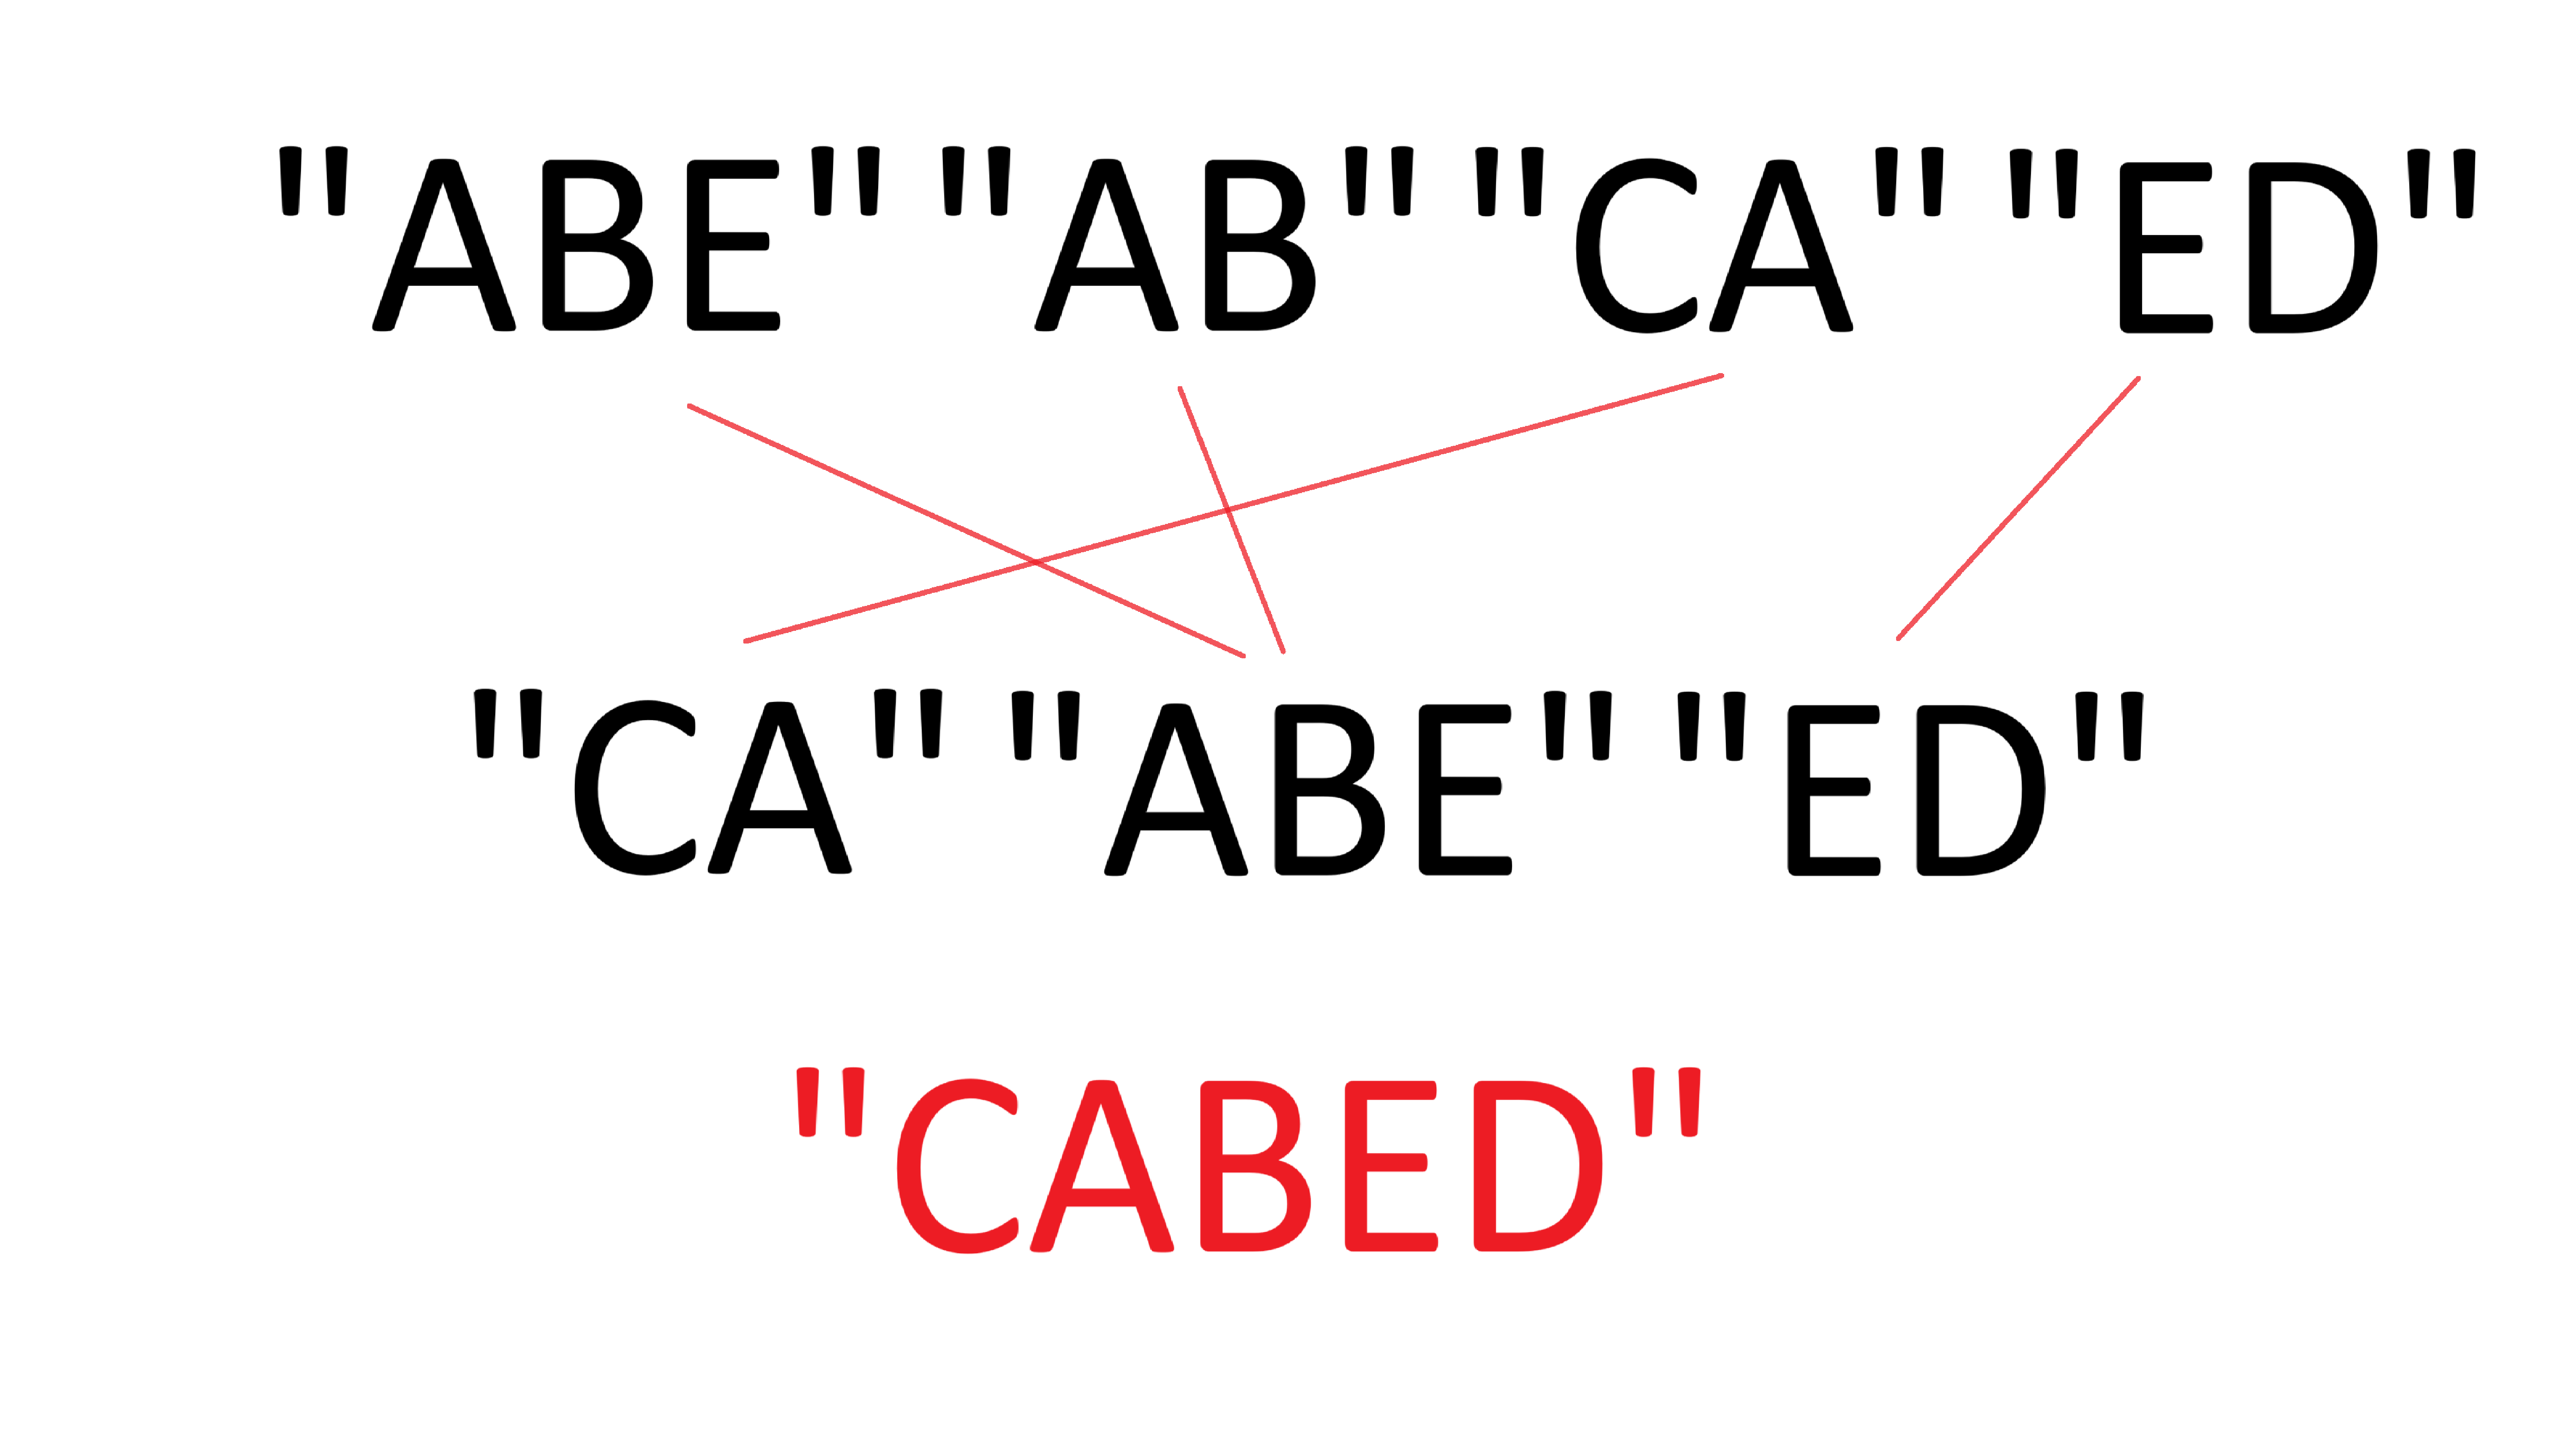
\includegraphics[scale=0.06]{img/example1.png}
    \caption{Пример надстроки}
\end{figure}
\begin{figure}[htbp]
    \center
    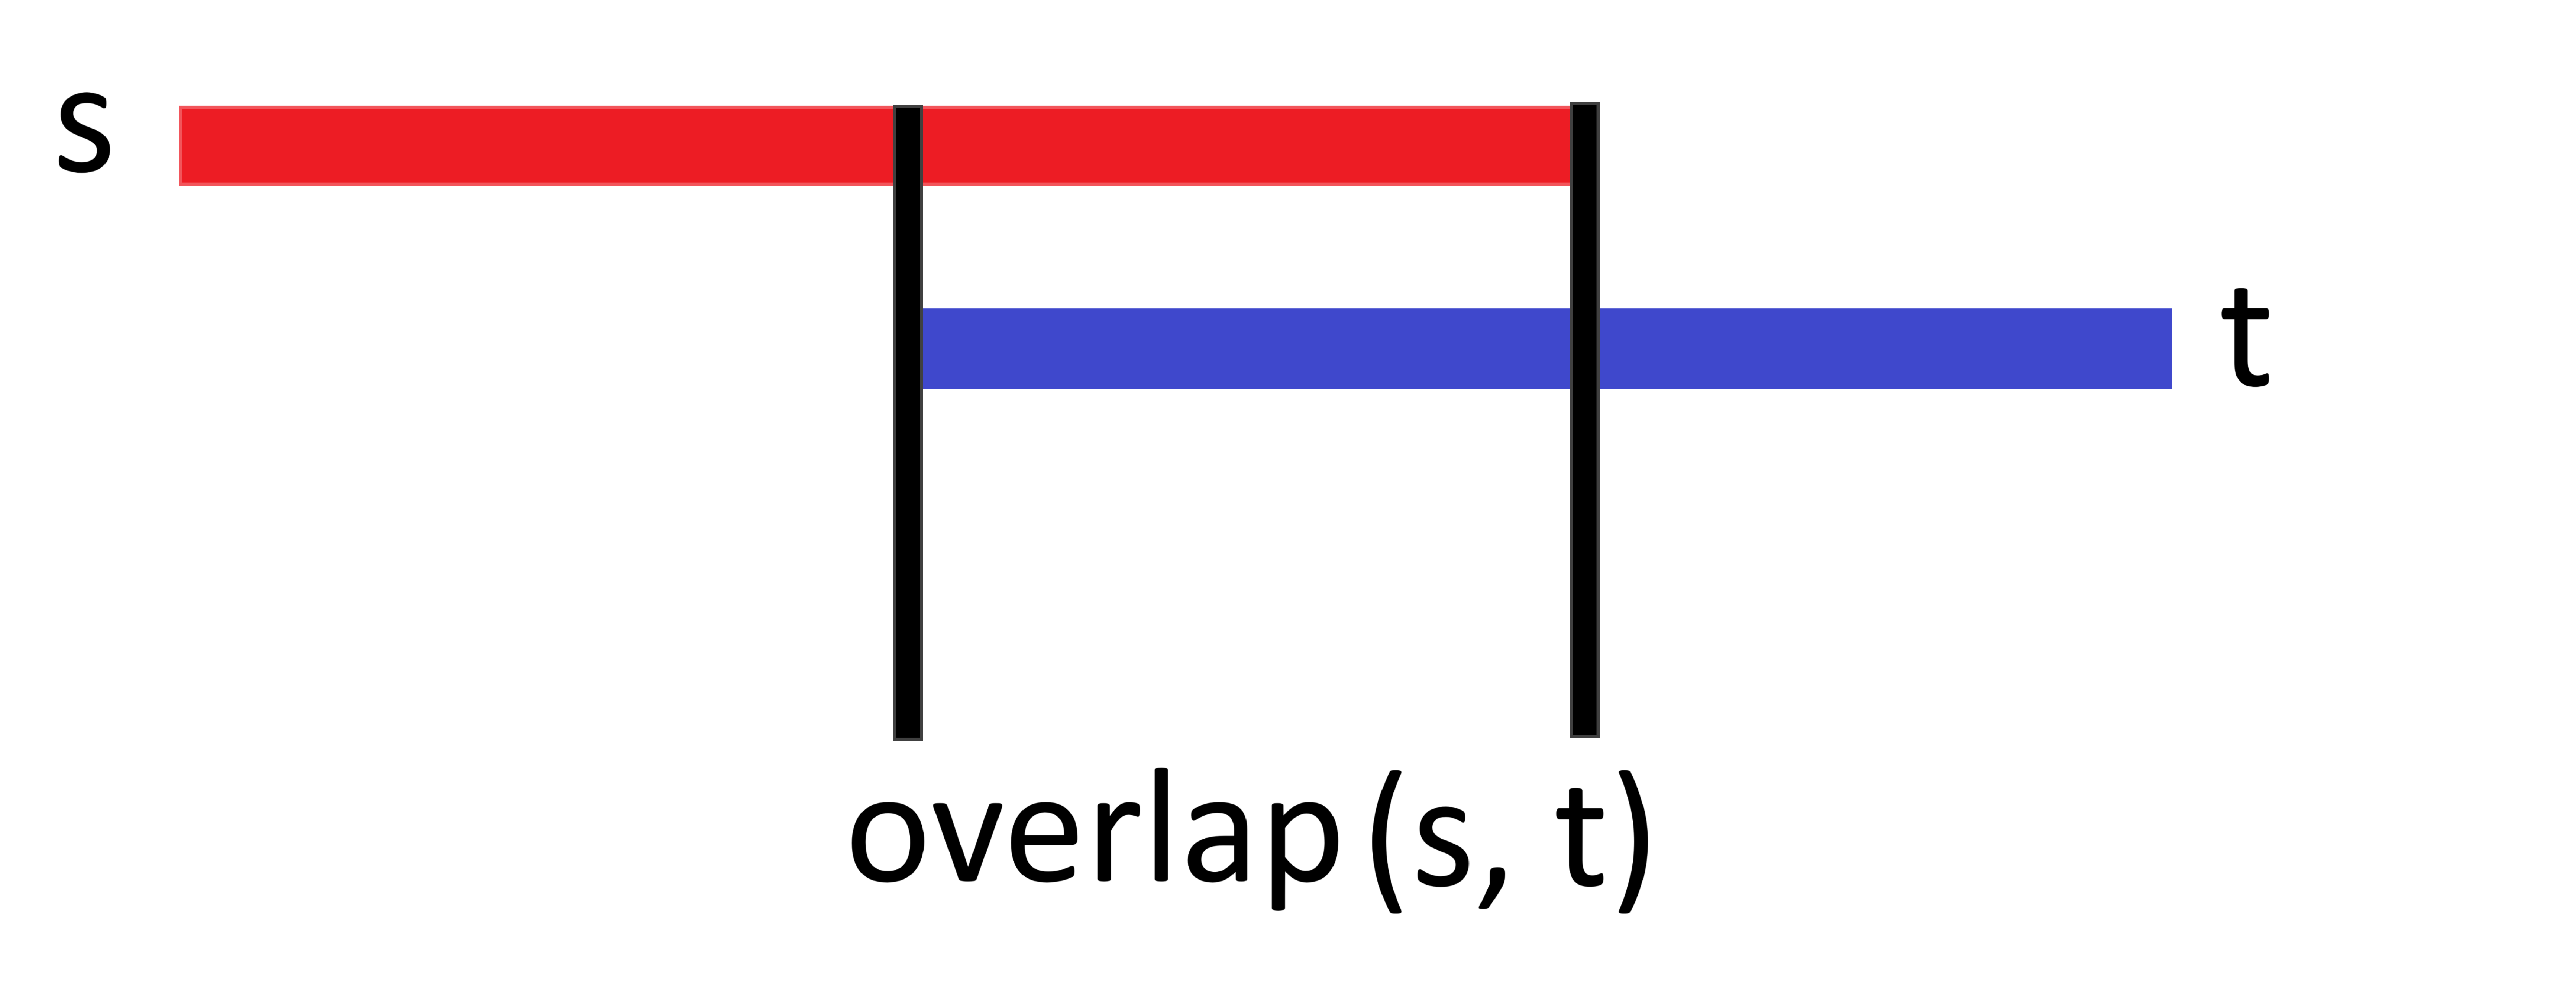
\includegraphics[scale=0.06]{img/example3.png}
    \caption{overlap}
\end{figure}


\newpage
\section{За какое время умеем решать}
\subsection{Перебор всех перестановок}
Заметим, что нам нужно максимимзировать количество {overlap}'oв, тогда чтобы гарантированно взять ту, в которой максимальное количество наложений, можно перебрать все перестановки из {n} элементов - строк и каждый раз собирать строку начиная слева направо. \newline
Такое решение будет работать за {O(n!n)}, что очень долго даже для n = 20. 

\subsection{Сведение к задачи коммивояжера}
Заметим, что нашу задачу можно представить в виде взвешанного ориентированного графа, где ребро {(u, v)} будет значить, что у строки {u} есть какой-то {overlap} с {v}, а вес на ребре будет обозначать какой именно длины будет этот {overlap}. К слову, это будет полный граф, так как у любых двух строк есть {overlap} хотя бы 0. \newline
После сведения, мы можем решить такую задачу при помощи динамического программирования по подмножествам, перебирая маску вершин, которые мы уже посетили и храня текущую.
\newline
Такое решение будет работать за {O(2^n n)}.


\end{document}
